\def\chapterabstract{In this chapter, we present a set of methods designed for tracking with high-order accuracy the propagation of surfaces in three dimensions with arbitrary geometric and topological complexity. Targeted applications are engineering and scientific problems for which a CAD (computer-aided design) model of the geometry is available, i.e. surface patches with high-order parameterizations as well as topological connectivity. Our method uses and maintains such a representation throughout the propagation. Validity of the dynamic boundary-representation model is ensured by handling geometric singularities. Examples are presented to demonstrate the accuracy of the pseudo-spectral method used for tracking each surface patch.
A strategy for deriving a dynamic surface mesh is finally proposed for applications such as Finite Element/Volume computations with body-fitted volume grids in domains with deforming boundaries. }

%\chapter{A chapter with short title}
%\chapter{Développement d'une méthode pseudo-spectrale pour le suivi d'un patch rectangulaire de surface}
%\chapter{Méthode pseudo-spectrale pour le suivi d'un patch rectangulaire de surface}
\chapter{Déformation de maillage surfacique}

%\epigraph{ Some fancy epigraph. }{ Anonym }

%\begin{abstract}
\printskip
\printchapapp
The work presented in this chapter focuses on surface propagation problems in industrial or scientific applications for which a CAD model of the geometry is available. The method presented in the following section takes this particular definition as a starting point and extends it to evolving geometries. \par
%\end{abstract}

Some \textbf{bold} text. Some \textit{italics} text. Some \emph{emphasized} text. Some \textsf{sans serif} text. Some \texttt{typewriter} text. {\color{myred} Some text in \textbf{red} \ldots} {\color{mygreen} Some text in \textbf{green} \ldots} \par
Mathcal $\mathcal{ABCDEFGHIJKLMNOPQRSTUVWXYZ}$.\\
Numbers: 1234567890, in math mode: $1234567890$.\\
{\scshape Small caps, in \textbf{bold}, in \textit{italics}.}

\newlength\TestLength
\setlength{\TestLength}{0pt}
\begin{figure}[htp]
  \centering
  \begin{tikzpicture}
    \node[rectangle,draw=red] (n) at (4,3) {abc};
    \getwidthofnode{\TestLength}{n}
    \node[anchor=north east] at (n.south west) {width = \the\TestLength};
    \getheightofnode{\TestLength}{n}
    \node[anchor=north west] at (n.south east) {height = \the\TestLength};
  \end{tikzpicture}
\end{figure}
TestLength = \the\TestLength.

\section{A section}

\paragraph*{Definition}
The $n$-th Chebyshev polynomial (of the first kind) $T_n$ is a polynomial of degree $n$ defined by
\begin{equation*}
	T_n \left(\cos \theta \right) = \cos n \theta.
    \label{def_cos}
\end{equation*}

For $x \in \chebinterval$, $T_0(x) = 1$, $T_1(x) = x$ and from the trigonometric identity $\cos n\theta + \cos (n-2)\theta = 2\cos \theta \cos (n-1)\theta $ the following recurrence relation can be derived
\begin{equation}
	T_{n}(x) = 2x T_{n-1}(x) - T_{n-2}(x) \quad, \quad n \geq 2.
    \label{eq:recurrence}
\end{equation}
Relation (\ref{eq:recurrence}) allows efficient evaluation of Chebyshev polynomials, e.g. via Clenshaw's algorithm \cite{clenshaw1955}. %The first five \cheb polynomials are plotted on {\modif Fig.} \ref{fig:poly_cheb}.
\par

On the interval $\chebinterval$, $T_n$ reaches its extremal values at the $n+1$ \textit{Chebyshev-Gauss-Lobatto} (CGL) points
\begin{equation*}
	\hat{x}_k = \cos \frac{k \pi}{n} \quad, \quad k = 0,\ldots,n.
\end{equation*}
\subsection{A subsection}

\begin{equation}
	\boldsymbol{f}(u,v) = \sum_{m = 0}^\infty \sum_{n = 0}^\infty \boldsymbol{c}_{mn} T_m(u) T_n(v) .
\end{equation}
Math macros\footnote{This is a footnote.} are tested in \Cref{sec:testmathmacros}.
\lipsum


\Cref{eq:recurrence} is an equation, \Cref{def_cos} is an equation, \Cref{fig0} is a figure. \fref{fig0} is a figure.

\begin{figure}
\centering
%\includegraphics[height=45mm]{/d/bandrieu/stck/Bureau/Figures/Degenerate/im_00}
\caption{Lagrangian transport may lead to mesh degeneracy.}
\label{fig0}
\end{figure}


\section{Another section}
\paragraph{Paragraph.}
\lipsum[1-7]

\begin{figure}
  \centering
  \begin{minipage}{0.4\textwidth}
    \centering
    %GRAPHIC 1
    
\includegraphics[height=45mm]{imr_trimmed_patch_xyz}
    \caption{Graphic 1 in a float} \label{fig:mult2}
  \end{minipage}
  \hfill
  \begin{minipage}{0.4\textwidth}
    \centering
    %GRAPHIC 2
    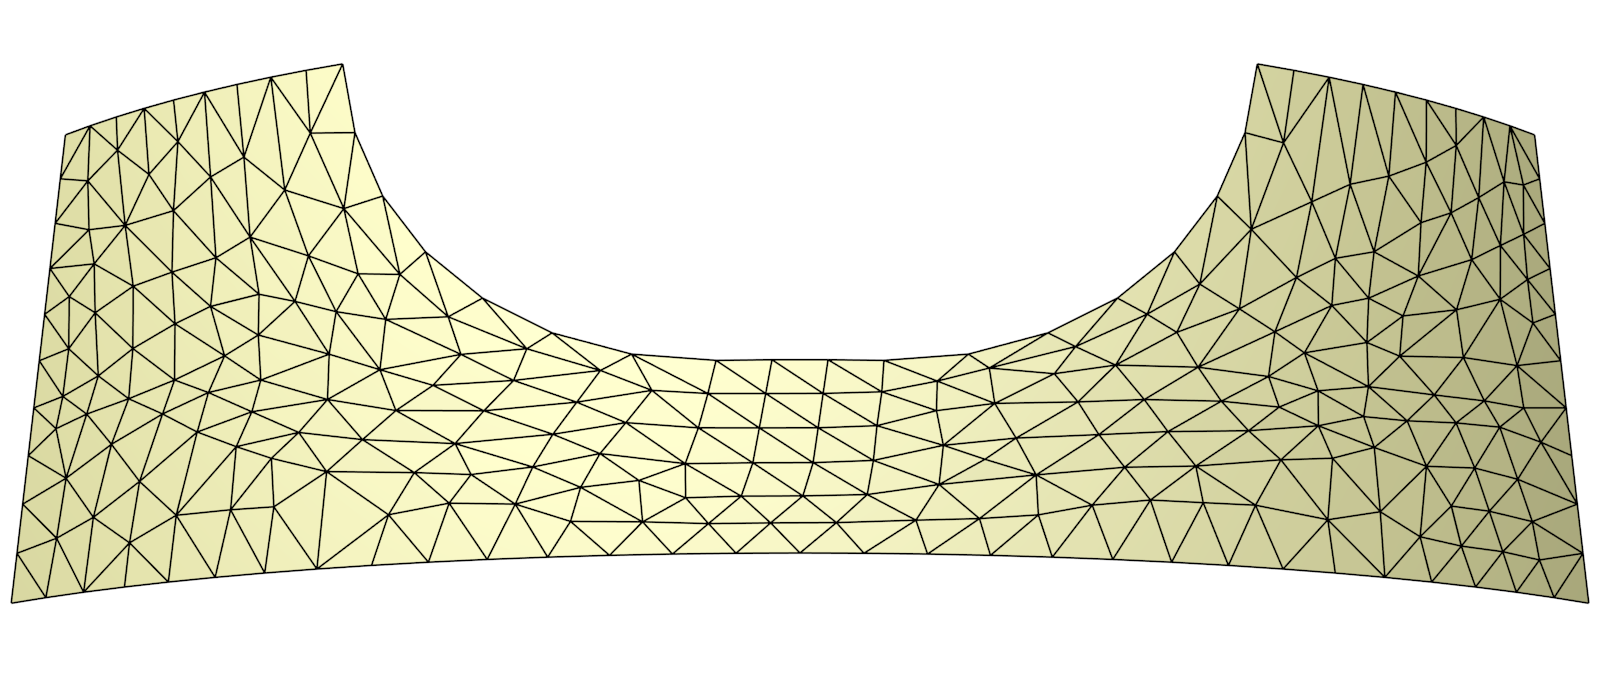
\includegraphics[height=20mm]{mesh_1c}
    \caption{Graphic 2 in same float} \label{fig:mult3}
  \end{minipage}
\end{figure}

\lipsum[8-15]

\begin{figure}
  \vspace{\onelineskip}
  \null\hfill\parbox{0.48\linewidth}{%
    \centering
    %Aligned to the center of the right figure
    
\includegraphics[height=45mm]{imr_trimmed_patch_xyz}
  }\hfill
  \parbox{0.48\linewidth}{%
    \centering
%     This is the right figure which is taller
%     than the first one (the one at the left)
	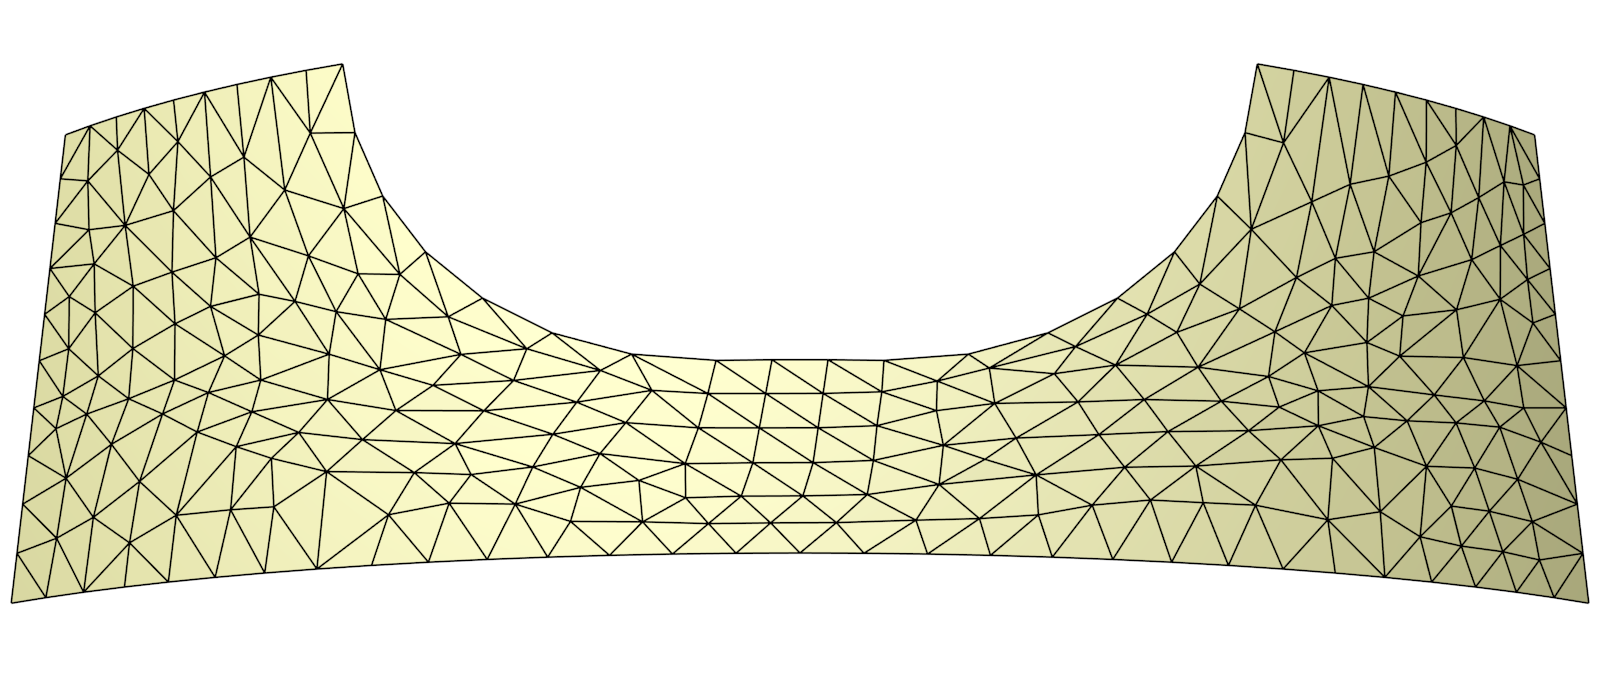
\includegraphics[height=20mm]{mesh_1c}
  }\hfill\null
  \vspace{\onelineskip}%\hrule
  \null\hfill\parbox[t]{0.48\linewidth}{%
  	\caption{Left figure}\label{fig:left1}%
  }\hfill
  \parbox[t]{0.48\linewidth}{%
    \caption{Right figure. This has more text than the adjacent
    caption (\ref{fig:left1}) so the heights are unequal}%
  	\label{fig:right1}%
  }\hfill\null
\end{figure}




\begin{figure}
  \centering
  \hspace*{\fill}
  \subbottom[Subfigure 1]{
  
\includegraphics[height=45mm]{imr_trimmed_patch_xyz}
  %\fbox{SUBFIGURE ONE}\label{sf:1}
  }
  \hfill
  \subbottom[Subfigure 2]{
  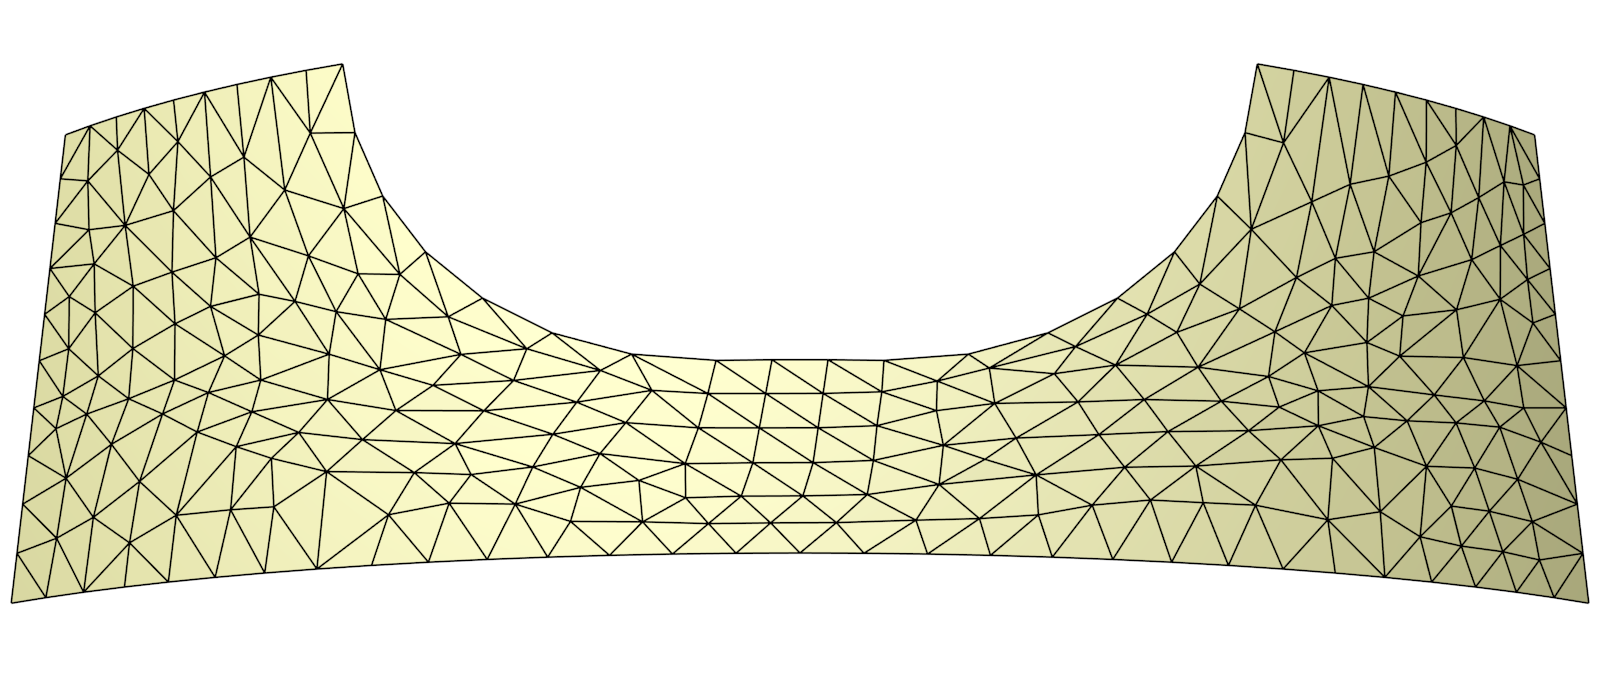
\includegraphics[height=20mm]{mesh_1c}
  %\fbox{SUBFIGURE TWO}\label{sf:2}
  }
  \hspace*{\fill}
  \caption{Figure with two subfigures} \label{fig:twosubfig}
\end{figure}


% \begin{figure}
%   \centering
%   \begin{minipage}{0.3\textwidth}
%     Some verbatim text
%     \subcaption{First text}
%   \end{minipage}
%   \hfill
%   \begin{minipage}{0.3\textwidth}
%     More verbatim text
%     \subcaption{Second text}
%   \end{minipage}
%   \caption{Verbatim texts}
% \end{figure}


\begin{figure}
  \centering
  \hspace*{\fill}
  \subbottom[Subfigure 1]{
  
\includegraphics[height=45mm]{imr_trimmed_patch_xyz}
  %\fbox{SUBFIGURE ONE}\label{sf:1}
  }
  \hfill
  \begin{tikzpicture}
      \useasboundingbox (0,0) rectangle(3cm,5cm);
	  \coordinate (a) at (5mm,45mm);
	  \draw[-latex] (a) to ([yshift=-3cm]a) node [left] {$x$};
	  \draw[-latex] (a) to node [above] {$y$} ([xshift=2cm]a);
  \end{tikzpicture}
  \hfill
  \subbottom[Subfigure 2]{
  
\includegraphics[height=45mm]{imr_trimmed_patch_xyz}
  %\fbox{SUBFIGURE TWO}\label{sf:2}
  }
  \hspace*{\fill}
  \caption{Figure with two subfigures} 
\end{figure}
